\documentclass[11pt,usenames, dvipsnames]{beamer}
\usetheme{Frankfurt}
\usepackage[utf8]{inputenc}
\usepackage[spanish]{babel}
\usepackage{xcolor}
% \usepackage{graphicx}
\usepackage{tikz}
\usepackage{subfig}
\usepackage{caption}
\usepackage{amsfonts}
\usepackage{multicol}
\usepackage{amsmath}
\usepackage{amssymb}

\usepackage{hyperref}

\usepackage{multirow, colortbl}
\usepackage{booktabs}

%\logo{%\includegraphics[height=0.34cm]{logo.png}\hspace{20pt}}
\definecolor{quantil}{rgb}{0.33, 0.41, 0.5}
\definecolor{lightseagreen}{rgb}{0.13, 0.7, 0.67}
\colorlet{quantil2}{quantil!59!black}
\colorlet{quantil3}{quantil!40!black}
\setbeamercolor{frametitle}{fg=white,bg=quantil2}
\setbeamercolor{section in head/foot}{bg=quantil3}
\setbeamercolor{author in head/foot}{bg=quantil2}
\setbeamercolor{date in head/foot}{fg=quantil2}
%\setbeamercolor{title}{quantil2}
\setbeamercolor{structure}{fg=quantil2}
\setbeamercolor{section number projected}{bg=lightseagreen,fg=white}
\setbeamercolor{enumerate item}{bg=lightseagreen}
\setbeamercolor{item projected}{bg=lightseagreen}

\newcounter{saveenumi}
\makeatletter
\let\@@magyar@captionfix\relax
\makeatother
\newcommand{\seti}{\setcounter{saveenumi}{\value{enumi}}}
\newcommand{\conti}{\setcounter{enumi}{\value{saveenumi}}}
\newcommand{\srcsize}{\@setfontsize{\srcsize}{3pt}{3pt}}

\author[creyesk]{Carlos Andrés Reyes\\
                 Quantil -- Universidad del Valle}

\title{Algunas aplicaciones de aprendizaje de máquinas \\
       en Colombia}
\date{Mieroles 17 de Octubre del 2018}

\begin{document}

{ % all template changes are local to this group.
    \setbeamertemplate{navigation symbols}{}
    \begin{frame}[plain]
        \begin{tikzpicture}[remember picture,overlay]
            \node[at=(current page.center)] {
                
\includegraphics[width=\paperwidth]{quantitle.png}
            };
        \end{tikzpicture}
     \end{frame}
}

\AtBeginSection[]{%
  \begin{frame}<beamer>
    \frametitle{Contenido}
    \footnotesize{
 \tableofcontents[currentsection,currentsubsection]}
  \end{frame}
  \addtocounter{framenumber}{-1}% If you don't want them to affect the slide number
}

\begin{frame}
\titlepage
\end{frame}

%%%%%%%%%%%%%%%%%%%%%%%%%%%%%%%%%%%%%%%%%%%%%%%%%%%%%%%%%%%%%%%

\begin{frame}{Una nueva cultura}
    \begin{itemize}
        \item En los últimos 2 años se ha producido y almacenado más información que en toda la historia de la humanidad.

        \item El acelarador de partículas en CERN puede generar varios petabytes ($10^6$ GB) de información diaria.

        \item Con los datos recolectados en las redes sociales Facebook nos conoce mejor que nuestros familiares.
    \end{itemize}
\end{frame}

\begin{frame}{Colombia no es la excepción}
    \begin{itemize}
        \item Los negocios buscan hacerle seguimiento a sus clientes e implementar politicas para retenerlos o hacerles ofertas.
        \item Las instuticiones financieras desean tener un cálculo más preciso de los riesgos a los que están expuestas.
        \item Los grupos de investigación tienen acceso a nuevas bases de datos para expandir sus proyectos.
    \end{itemize}
\end{frame}

\begin{frame}{Gapmaps}
    \begin{itemize}
        \item Aproximadamente 60,000 artículos para cada tema.
        \item ¿Podemos clasificar los artículos en un número dado de tópicos?
        \item ¿Cuales son los tópicos más interesantes?
        \item ¿Que metodologías se utilizan en los artículos?
    \end{itemize}
        \begin{figure}
        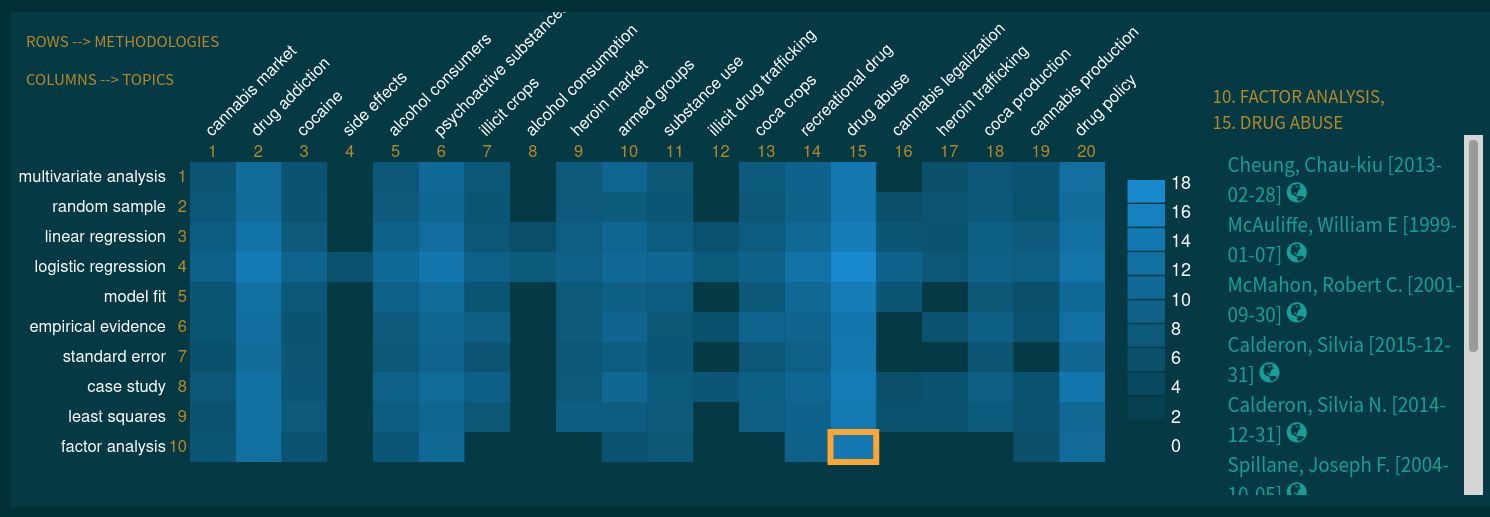
\includegraphics[width=\textwidth]{figures/gapmap}
        \caption{\href{http://seixas.quantil.co/api/site/}{Gapmap} para 60,000 artículos sobre drogas.} 
    \end{figure}
\end{frame}

\begin{frame}{Riesgo de Crédito}
    \begin{itemize}
        \item Se desea calcular la probabilidad de que alguien incumpla con los pagos de un crédito.
        \item Se conocen algunos datos del cliente al momento de pedir el crédito (variables demográficas, comportamiento crediticio). 
        \item Se hace un seguimiento del comportamiento de pago del cliente para así calcular su probabilidad de incumplimiento en cualquier momento.
    \end{itemize}
\end{frame}

\begin{frame}{Redes neuronales recurrentes para las series de tiempo}
    \begin{figure}
        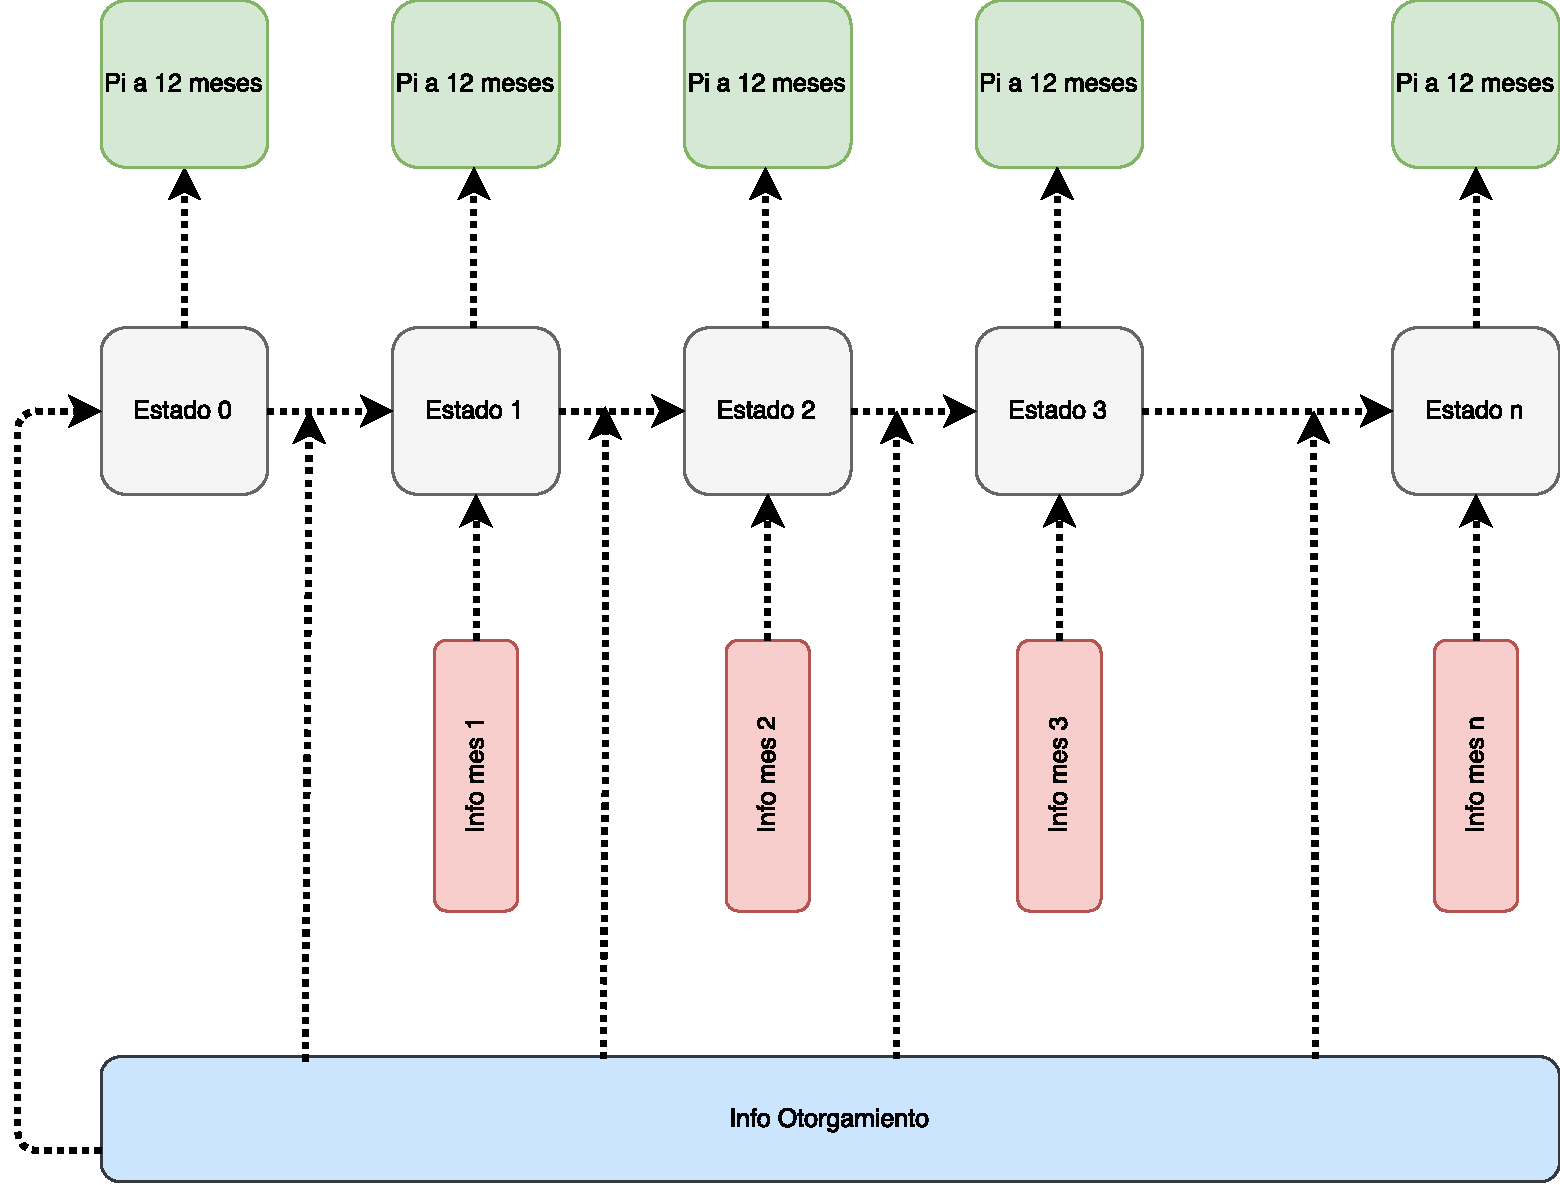
\includegraphics[width=0.7\textwidth]{figures/SARC} 
        \caption{Diagrama de una red neuronal recurrente en el ámbito de riesgo de crédito.}
    \end{figure}
\end{frame}


\begin{frame}{Neuronas LSTM (Long Short Term Memory)}
    \begin{figure}
      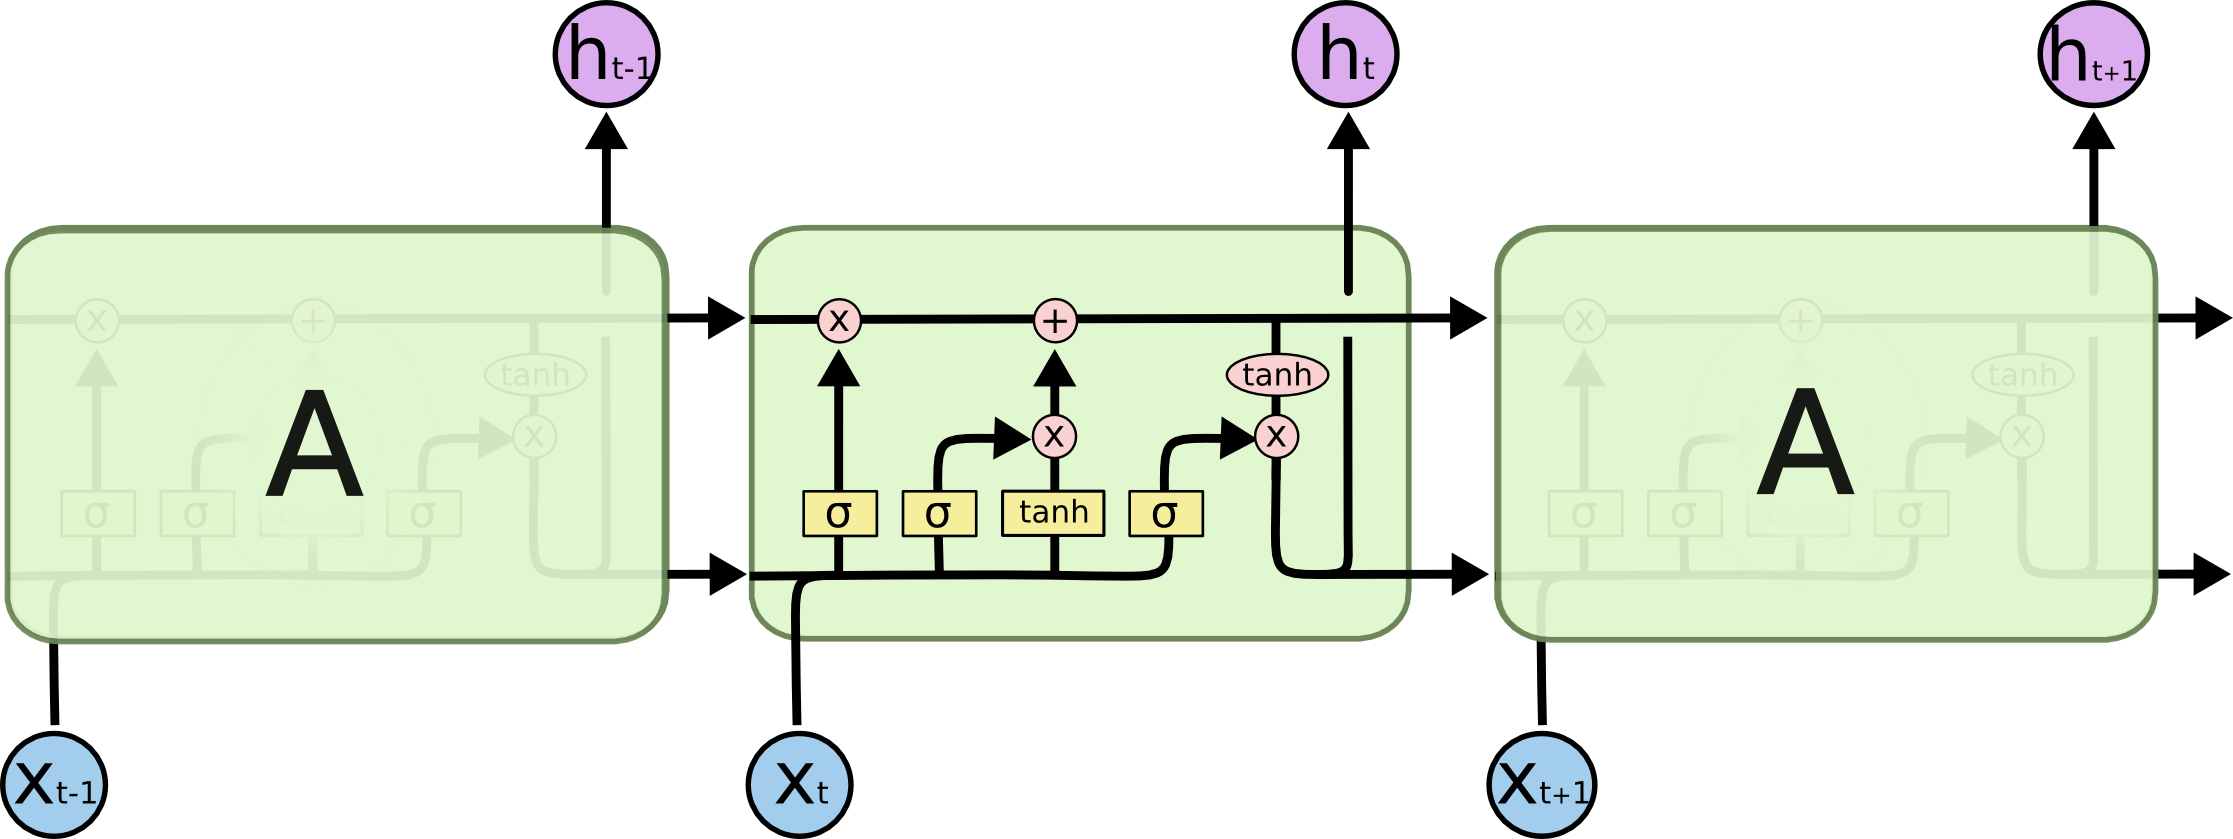
\includegraphics[width=\textwidth]{figures/lstm}
      \caption{Understanding LSTM Networks, Christopher Colah 2015.}
    \end{figure}
\end{frame}



\begin{frame}{Comportamiento de las redes sociales}
    \begin{itemize}
        \item Durante el proceso de paz se presenció una alta polarización en las redes sociales. 
    \end{itemize}
    \begin{figure}
        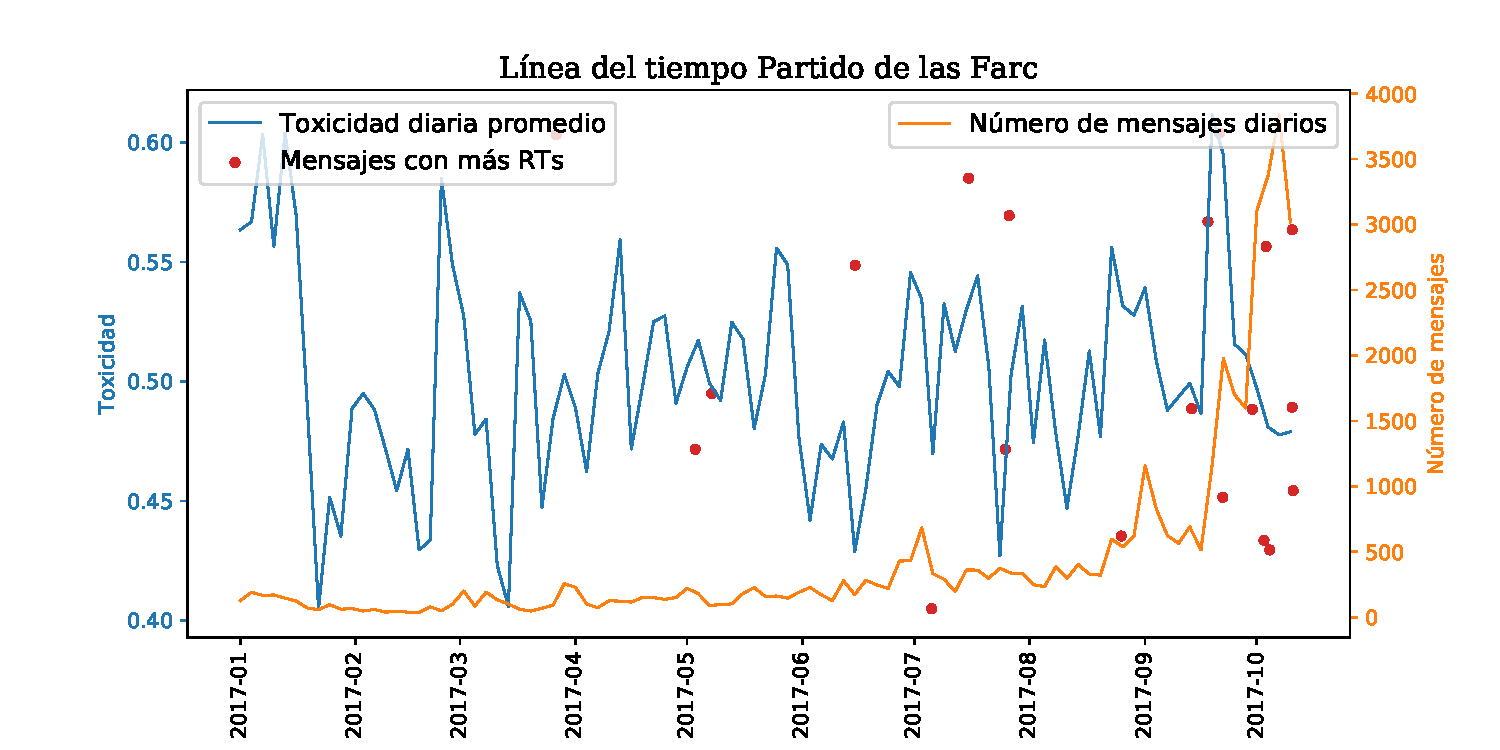
\includegraphics[width=\textwidth]{figures/tweets}
        \caption{Linea de tiempo de tweets y su toxicidad.}
    \end{figure}
\end{frame}

\begin{frame}{Análisis de sentimiento}
Utilizando Algoritmos de clasificación como regresión logística o árboles aleatorios se identifican los mensajes tóxicos y sus características. Lo mismo se puede hacer para los perfiles de los usuarios.
    \begin{figure}
        \centering
        \begin{minipage}{0.49\textwidth}
            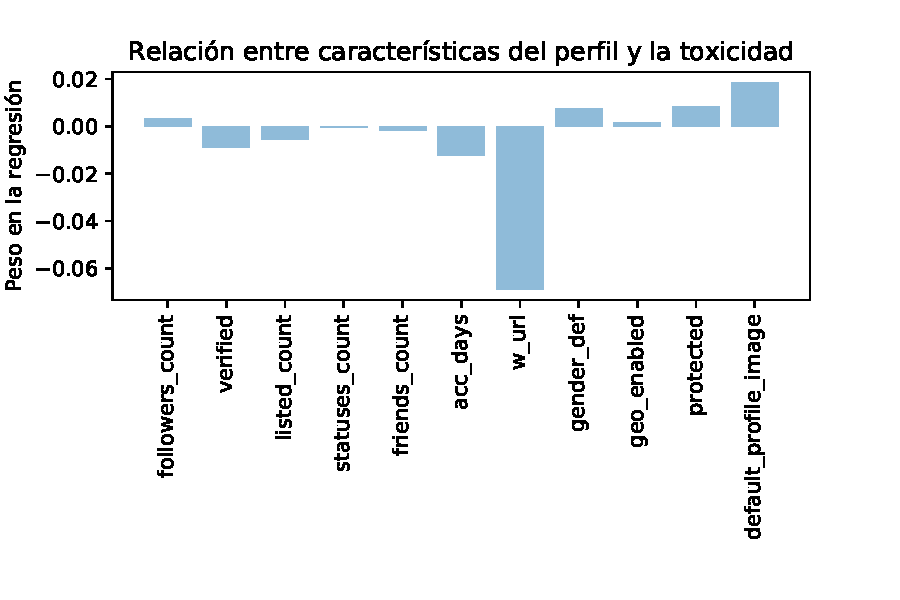
\includegraphics[width=1\linewidth]{figures/sentimientoUsuario}
        \end{minipage}
        \begin{minipage}{0.49\textwidth}
            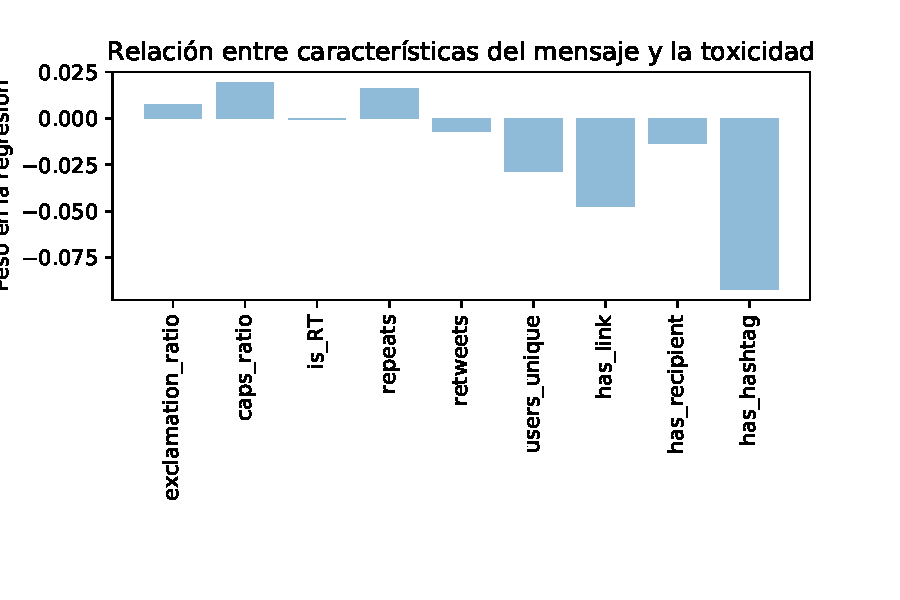
\includegraphics[width=1\linewidth]{figures/sentimientoMensaje}
        \end{minipage}    
    \end{figure}
\end{frame}

\begin{frame}{Identificación de grupos claves}
    \centering
    \begin{table}
    \resizebox{.65\textwidth}{!}{
    \begin{tabular}{lrrrrrrrrr}
        \toprule
        {} & {} & followers\_count & tweets\_day & verified & msg\_count & mean\_repeats & mean\_unique & \multicolumn{2}{l}{retweets} \\
        {cluster} &              count &            mean &       mean &     mean &      mean &         mean &        mean &     mean & score \\
         \midrule
        0       &              33280 &         2,398.4 &        5.6 &      0.0 &       1.5 &          1.1 &         0.3 &      1.0 &   0.0 \\
        1       &                 36 &         9,008.6 &       25.5 &      0.0 &       9.9 &        134.0 &        18.5 &      0.1 &  \cellcolor{ForestGreen!25} 0.5 \\
        2       &                657 &       196,167.1 &       24.2 &      1.0 &       2.2 &          1.6 &         0.6 &     15.0 &   0.0 \\
        3       &                 26 &       122,647.2 &      930.2 &      0.2 &       4.9 &          7.2 &         4.0 &      1.3 &  \cellcolor{ForestGreen!50} 1.0 \\
        4       &                 27 &       248,205.2 &       13.1 &      0.6 &       3.9 &          3.3 &         2.0 &    507.5 &   0.0 \\
        5       &                 17 &         7,320.0 &      128.0 &      0.0 &     151.9 &          1.9 &         0.5 &      1.2 &  \cellcolor{ForestGreen!25} 0.5 \\
        6       &                 37 &     3,917,430.7 &      160.9 &      1.0 &       8.8 &          4.7 &         2.6 &     36.8 &   0.0 \\
        7       &                433 &        29,281.2 &      157.2 &      0.0 &       3.5 &          3.1 &         1.9 &      2.0 &  \cellcolor{ForestGreen!25} 0.5 \\
        8       &                 64 &           937.6 &        5.0 &      0.0 &       1.2 &        109.2 &       103.9 &      1.2 &   0.0 \\
        9       &                517 &         2,392.9 &       22.3 &      0.0 &      23.5 &          1.7 &         0.2 &      2.2 &   0.0 \\
        10      &                  1 &    16,237,961.0 &       40.6 &      1.0 &       1.0 &          3.0 &         3.0 &     53.0 &   0.0 \\
        11      &                343 &         2,552.6 &       25.6 &      0.0 &       1.4 &         27.5 &        26.4 &      0.5 &   \cellcolor{ForestGreen!25} 0.5 \\
        12      &                133 &        87,865.7 &       16.1 &      0.3 &       3.8 &          1.6 &         0.8 &    171.1 &   0.0 \\
        \bottomrule
    \end{tabular}
    }
    \caption{Identificación de Bots}
    \end{table}

    \begin{table}
    \resizebox{.65\textwidth}{!}{
    \begin{tabular}{lrrrrrrrr}
        \toprule
        {} & & followers\_count & verified & friends\_count & following & listed\_count & \multicolumn{2}{l}{retweets} \\
        cluster &              count &            mean &     mean &          mean &      mean &         mean &     mean & score \\
        \midrule
        0       &              34641 &         2,421.1 &      0.0 &         759.2 &       0.0 &         18.8 &      1.0 &     0 \\
        1       &                 50 &     1,638,087.4 &      0.9 &       5,776.8 &       0.0 &      5,367.6 &     25.2 &    \cellcolor{ForestGreen!50} 1 \\
        2       &                 82 &       276,594.6 &      0.3 &       2,439.2 &       1.0 &        603.2 &     29.7 &   \cellcolor{ForestGreen!50}  1 \\
        3       &                608 &       124,496.3 &      1.0 &       2,523.2 &       0.0 &        515.9 &     13.9 &  \cellcolor{ForestGreen!50}   1 \\
        4       &                 19 &     4,846,204.2 &      1.0 &      19,734.2 &       0.4 &     14,794.1 &     45.9 &   \cellcolor{ForestGreen!50}  1 \\
        5       &                  3 &     1,696,799.0 &      0.7 &     673,827.7 &       0.0 &      4,005.7 &      3.6 &     0 \\
        6       &                116 &        85,662.6 &      0.3 &       3,333.3 &       0.0 &        305.6 &    191.6 &   \cellcolor{ForestGreen!50}  1 \\
        7       &                  2 &    11,346,163.0 &      1.0 &         798.0 &       0.0 &     52,453.5 &     36.9 &   \cellcolor{ForestGreen!50}  1 \\
        8       &                 20 &       300,493.6 &      0.6 &       2,144.7 &       0.1 &        890.5 &    560.3 &  \cellcolor{ForestGreen!50}   1 \\
        9       &                 30 &       226,817.3 &      0.1 &     109,075.9 &       0.0 &      1,243.8 &     24.0 &     0 \\
        \bottomrule
    \end{tabular}
    }
    \caption{Famosos}
    \end{table}
\end{frame}

\begin{frame}{Análisis de redes}
    \begin{figure}
        \centering
        \begin{minipage}{0.49\textwidth}
            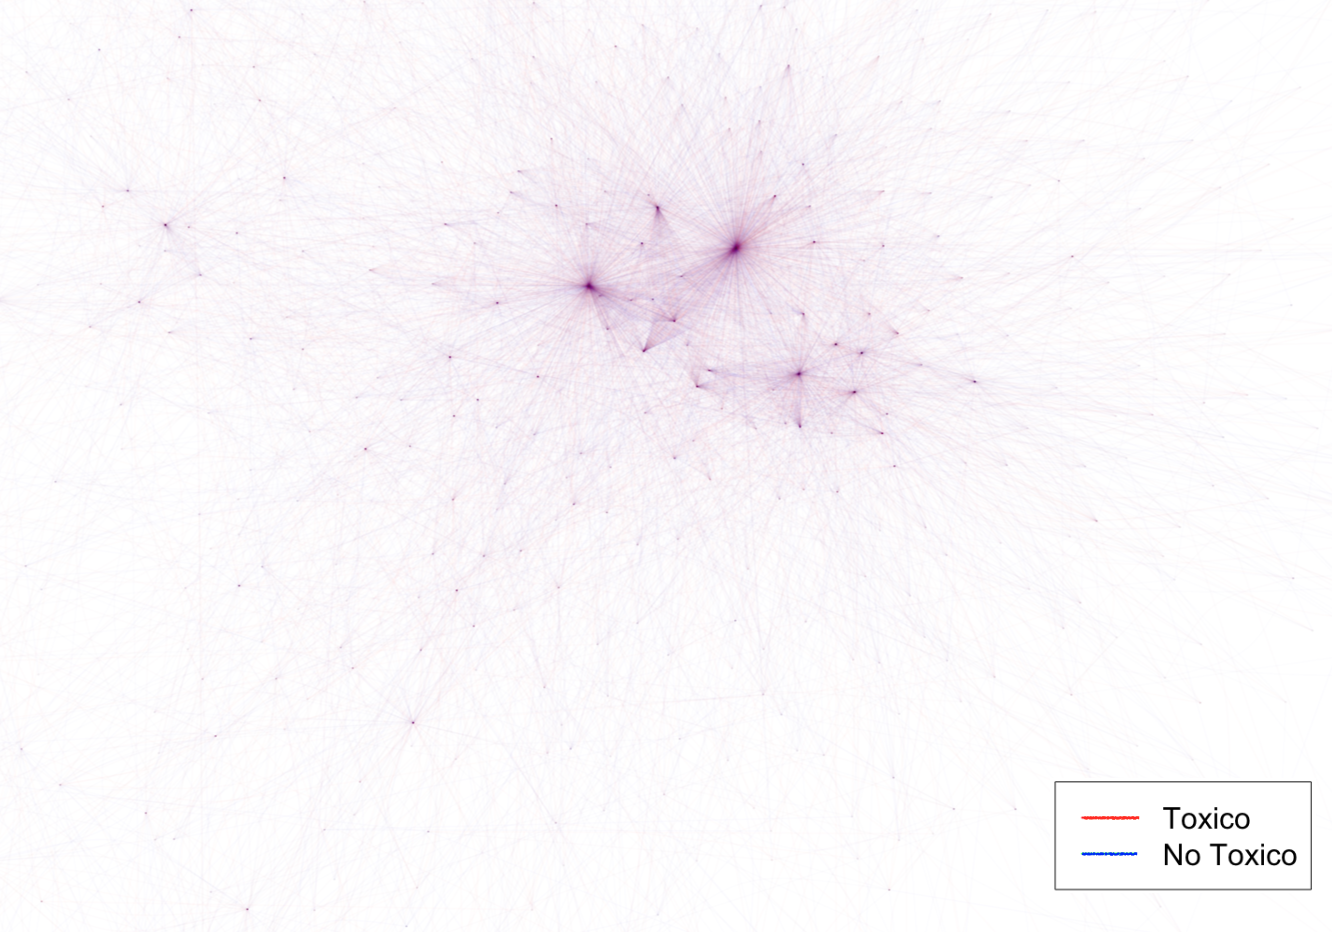
\includegraphics[width=0.6\textheight]{figures/red_farc}
        \end{minipage}
        \begin{minipage}{0.49\textwidth}
            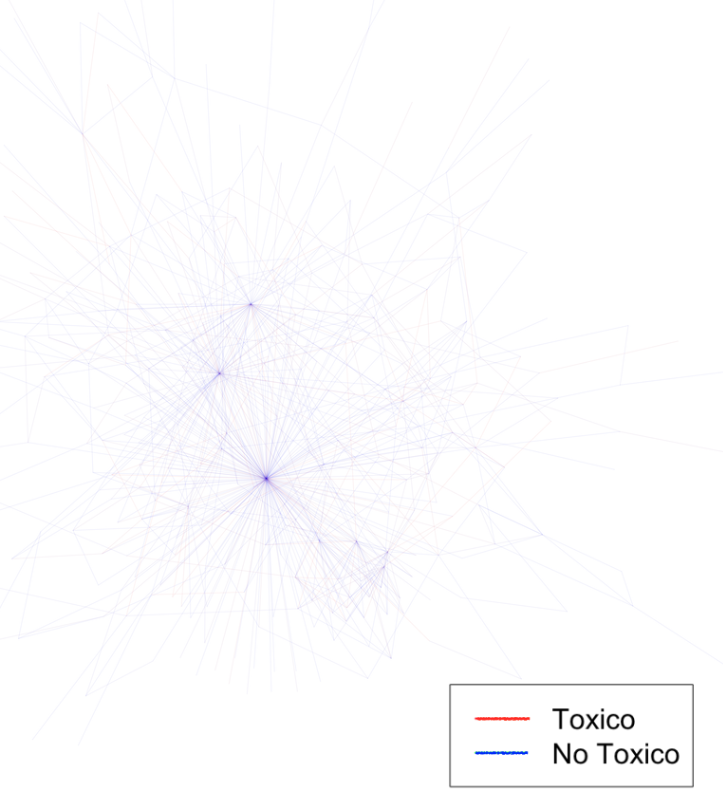
\includegraphics[width=0.5\textheight]{figures/red_genero}
        \end{minipage}    
        \caption{Redes de conversaciones en Twitter para dos casos. Izquierda: Partido de las Farc. Derecha: Genero (caso Andrea Guerrero.)}
    \end{figure}
\end{frame}


\begin{frame}{Arte con redes neuronales profundas}
    \begin{figure}
        \centering
        \begin{minipage}{0.49\textwidth}
            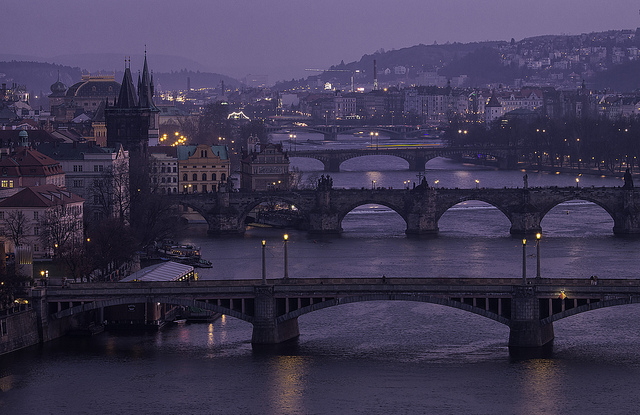
\includegraphics[height=0.45\textheight]{figures/prag}
             \caption{Imágen de contenido}
        \end{minipage}
        \begin{minipage}{0.49\textwidth}
            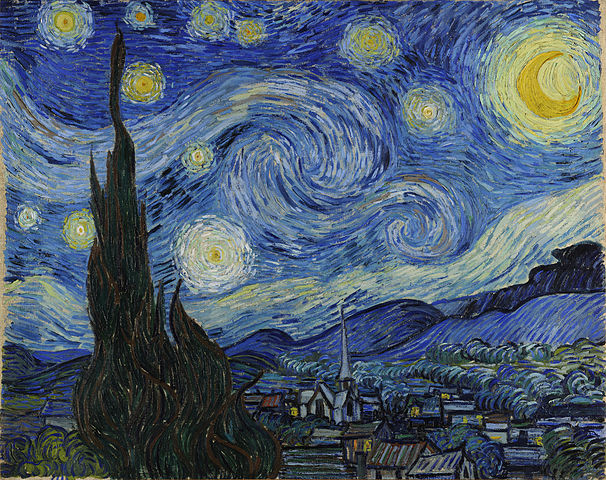
\includegraphics[height=0.45\textheight]{figures/star}
            \caption{Imágen de estilo}
        \end{minipage}    
    \end{figure}
\end{frame}

\begin{frame}{Resultado}
    \begin{figure}
        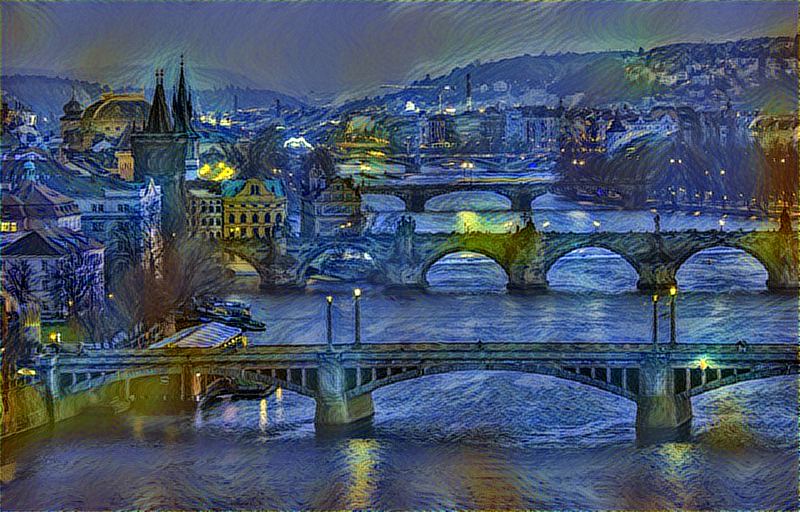
\includegraphics[width=\textwidth]{figures/prag_deep}
    \end{figure}
\end{frame}

\begin{frame}{Arte con redes neuronales profundas}
    \begin{figure}
        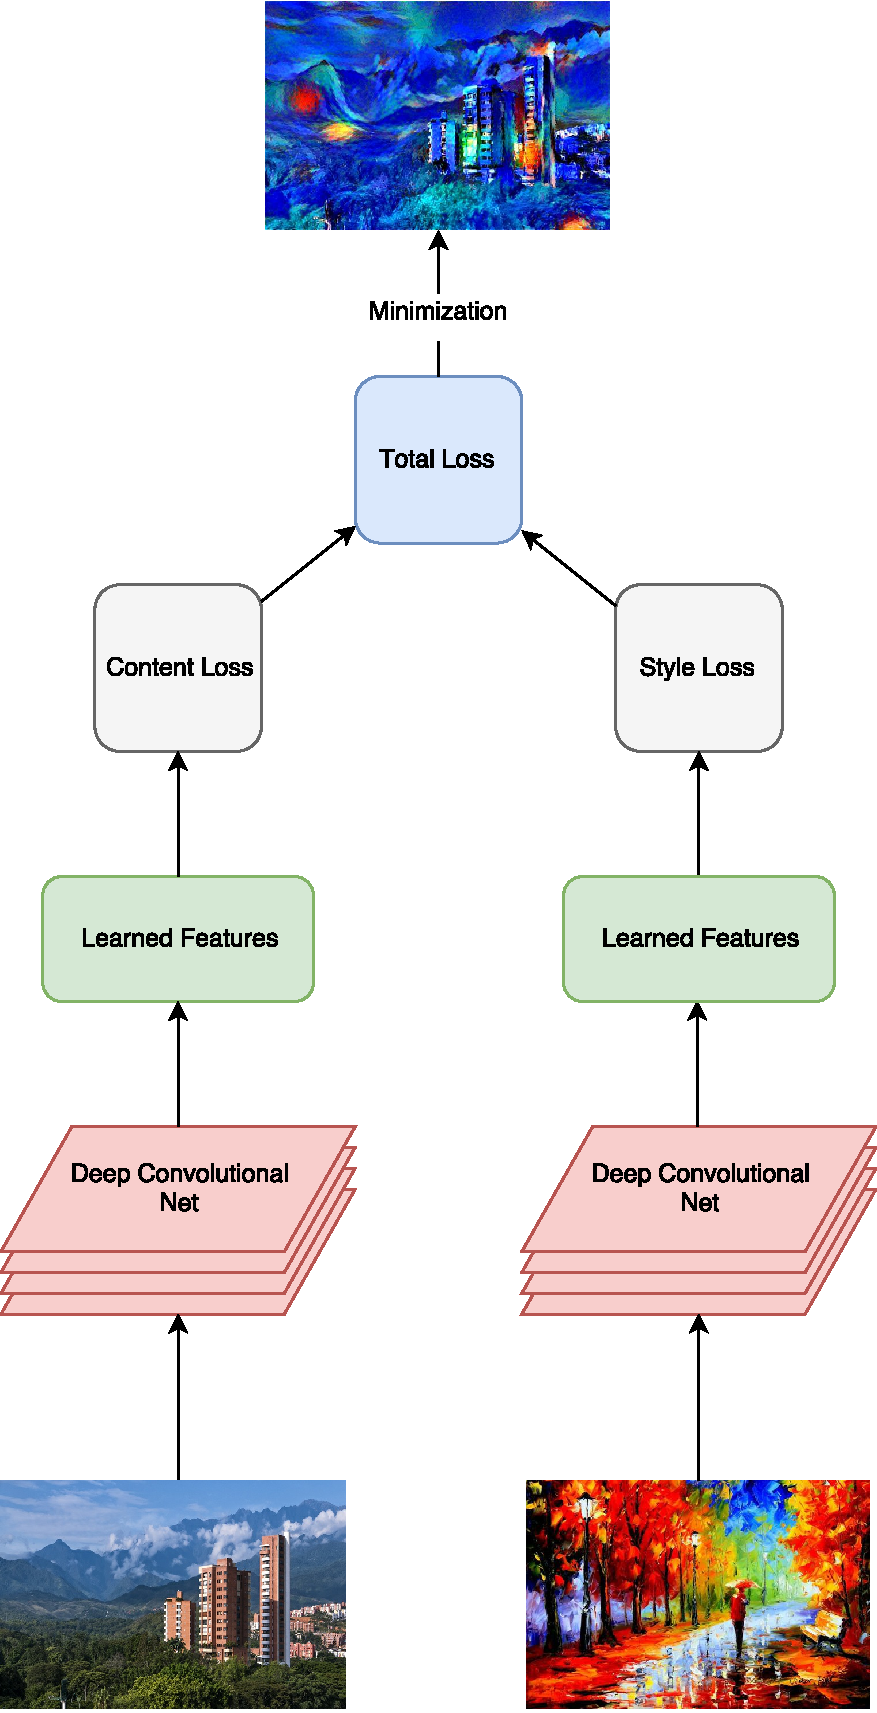
\includegraphics[height=0.8\textheight]{figures/art}
    \end{figure}
\end{frame}



{ % all template changes are local to this group.
    \setbeamertemplate{navigation symbols}{}
    \begin{frame}[plain]
        \begin{tikzpicture}[remember picture,overlay]
            \node[at=(current page.center)] {
                
\includegraphics[width=\paperwidth]{gracias.png}
            };
        \end{tikzpicture}
     \end{frame}
}
\end{document}